\section{A pattern is a counting map and an ink function}
\label{sec:object}
\label{sec:field}
\label{sec:catalog}

A layer, stripped of its raster, is a countable family of curves
$\{\gamma_n\}$: the $n$th line, the $n$th ring, the $n$th turn of a spiral.
We never represent that family as geometry. We represent it as a pair
$(\cnt,F)$.

\begin{definition}[Counting map and ink]
A \emph{counting map} is a function $\cnt\colon M\to\T^K$ from the drawing
plane (or a punctured subset of it) to a $K$-torus. Each coordinate
$\idx_i$ of $\cnt=(\idx_1,\dots,\idx_K)$ names a member of one family,
fractionally, so that $\gamma_n=\idx_i^{-1}(n)$ wherever the coordinate
is single-valued. The gauge lattice $\Z^K$ absorbs the arbitrary choice
of who is member zero. $K$ is the pattern's \emph{rank}: one for a
scalar family, two for a lattice, $K$ for a stack.
An \emph{ink function} $F\colon\T^K\to[0,1]$ paints the torus. The
drawn image is $F\circ\cnt$.
\end{definition}

The distance field $d(p)=\min_n\mathrm{dist}(p,\gamma_n)$ is the leading
term of $F$; a stroke of half-width $h$ is the sublevel
$\{d\le h\}$, antialiased. The index field of the current paper is one
coordinate of $\cnt$. Superposition of $K$ layers is the joint map
$\cnt=(\idx_1,\dots,\idx_K)$ with $F$ the union of the per-layer inks.
Everything that follows is a statement about this pair.

Two axes organize the catalog. Rank is one of them. The other is how
integrable $\cnt$ is.

\begin{center}
\small
\begin{tabular}{@{}lll@{}}
  \toprule
  & rank $1$ & rank $2$ \\
  \midrule
  exact
    & the nine phase families
    & the three lattices \\
  defect
    & radial pencil; $\theta$ fields
    & --- \\
  fold
    & walking families
    & --- \\
  \bottomrule
\end{tabular}
\end{center}

\emph{Exact.} $\cnt$ is the graph of a global scalar (or pair of
scalars). The nine phase families of Table~\ref{tab:catalog} are all
the same family: parallel lines, precomposed with a field. Circles are
lines of $r$, parabolas are lines of $y-ax^2$, spirals are lines of
$r-b\theta$. The space of exact rank-$1$ patterns is an affine space
over scalar fields, which is why \S\ref{sec:beyond} can encode a field
as a difference of patterns. Rank $2$ is the three lattices: two
generators, ink on the torus that decides whether a honeycomb or a
triangle lattice is drawn. Kind lives in $F$; geometry lives in
$\cnt$. That is why the envelope's ink weights had to exist
(\S\ref{sec:envelope}).

\emph{Defect.} The counting form is closed but has periods. $\idx$ is
circle-valued, with winding. The radial pencil of $N$ undirected lines
through the origin is not an exception to the theory. Its index is
$N\theta/\pi$, a pure winding field, so the pencil is the charge-$2N$
defect of the line family. A field containing \texttt{theta} mints the
same object (\S\ref{sec:defects}): \texttt{theta/tau} at integer
amount $A$ inserts $A$ extra members, a fork.

\emph{Fold.} There is no global form. The local index tears along
envelope curves. Walking families live here: member $n$ is the shape of
radius $ns+\varphi$, displaced by $n\delta$ and turned by $n\theta$,
and no formula in $p$ has those curves as its level sets. Search is
the price of non-integrability; the certificate of
\S\ref{sec:inverse} is the interest rate.

\subsection{Phase, index, distance}

Most exact families are the level sets of a single scalar \emph{phase}
function $\ph$, kept in world units so that member $n$ is
$\{\ph=ns+\varphi\}$. Then
\begin{equation}
  \idx(p) = \frac{\ph(p)-\varphi}{s},
  \qquad
  d(p) \;\simeq\; \frac{\mathrm{pd}\!\left(\ph(p)-\varphi,\; s\right)}{\lVert\nabla\ph(p)\rVert},
  \label{eq:eikonal}
\end{equation}
where $\mathrm{pd}(v,s)=\min_{k\in\Z}|v-ks|$ is the distance from $v$
to the lattice $s\Z$. The division is Taubin's first-order distance
approximation for implicit curves~\cite{Taubin1994Distance}, applied
to a phase residual. Both fields are one line of shader code.

Table~\ref{tab:catalog} is the list. Thirteen families ship; nine of
them are this equation with the $\ph$ of a row. The four that are not
are the defect and fold rungs, and the rank-$2$ lattices.

\begin{table*}[t]
  \centering
  \caption{\figlead{The nine phase families.} Each row is a complete
  specification: substitute $\ph$ and $\lvert\nabla\ph\rvert$ into
  \eqref{eq:eikonal} and the layer renders; the square, triangle and
  hexagon rows are the $N=4$, $3$, $6$ instances of the $N$-gon row, written
  out because their support forms are transcendental-free. $\omega=2\pi f/32$ so that
  $f=1$ is one wave cycle per $32$ world units; $a=B/100$ for a bend slider $B$;
  $b=Ms/2\pi$ with $M=\max(1,\mathrm{round}(\lvert B\rvert/s))$ the number of
  spiral arms. The three concentric shapes are the support function of the
  generating polygon, which is the observation \S\ref{sec:walking} builds on.}
  \label{tab:catalog}
  \small
  \begin{tabular}{@{}llll@{}}
    \toprule
    Family & $\ph(p)$ & $\lvert\nabla\ph(p)\rvert$ & Notes \\
    \midrule
    Parallel lines
      & $\langle p,u\rangle$
      & $1$
      & $u=(\cos\alpha,\sin\alpha)$; pitch $s$ \\
    Concentric circles
      & $\lVert p\rVert$
      & $1$
      & \\
    Concentric squares
      & $\max(\lvert x\rvert,\lvert y\rvert)$
      & $1$
      & $L^\infty$; support function of the square \\
    Concentric triangles
      & $\max\!\left(x,\ \tfrac{\sqrt3}{2}\lvert y\rvert-\tfrac{x}{2}\right)$
      & $1$
      & support function of the triangle \\
    Concentric hexagons
      & $\max\!\left(\lvert x\rvert,\ \tfrac{\lvert x\rvert}{2}+\tfrac{\sqrt3}{2}\lvert y\rvert\right)$
      & $1$
      & support function of the hexagon \\
    Concentric $N$-gon
      & $\lVert p\rVert\cos\!\big(\mathrm{wrap}(\theta_p,\tfrac{2\pi}{N})\big)$
      & $1$
      & $\theta_p=\mathrm{atan2}(y,x)$ \\
    Wave
      & $x-A\sin(\omega y+\ph_0)$
      & $\sqrt{1+A^2\omega^2\cos^2(\omega y+\ph_0)}$
      & $A$ amplitude, $f$ frequency, $\ph_0$ phase \\
    Parabola
      & $y-a x^2$
      & $\sqrt{1+4a^2x^2}$
      & opens up; $a=0$ is horizontal parallels \\
    Hyperbola
      & $\sqrt{\lvert x^2-y^2\rvert}$
      & $\lVert p\rVert/\sqrt{\lvert x^2-y^2\rvert}$
      & rectangular; $n\ge1$, so no member through $0$ \\
    Spiral
      & $\lVert p\rVert-b\,\theta_p$
      & $\sqrt{1+b^2/\lVert p\rVert^2}$
      & Archimedean; $b=0$ is concentric circles \\
    \bottomrule
  \end{tabular}
\end{table*}

Three remarks on the table, each a bug we shipped.

\paragraph{The gradient column is not decoration.} For the first six rows it is
$1$ and can be dropped. For the last four it is not, and dropping it thins every
stroke by the same factor the family is steep by. We had shipped that bug in
three of the four; \S\ref{sec:eikonal} reports the measurement.

\paragraph{Some families exclude an index.} The hyperbola's $n=0$ member would be
the degenerate pair $x=\pm y$, and $\lvert\nabla\ph\rvert$ blows up there, so the
family starts at $n=1$. The spiral's $\ph$ has a branch cut wherever
$\mathrm{atan2}$ does; it closes only if the arm count $M$ is an integer, which is
why $M$ is rounded rather than passed through. Both are the kind of detail that a
raster pipeline hides in the resampling and a field pipeline exposes on the
first frame.

\paragraph{Three of the rows are support functions.} The square, triangle and
hexagon entries are all $\rad(q)=\max_k\langle q,n_k\rangle$ over the outward
facet normals, written out. So is the $N$-gon row, in its trigonometric form. This
is not a coincidence and it is not only a way to avoid an $\mathrm{atan2}$:
\S\ref{sec:walking} shows that the same object supplies the constants that make
the fold rung tractable.

The radial pencil has a distance rather than a phase,
\begin{equation}
  d(p)=\max\!\Big(\lVert p\rVert\,\big\lvert\sin\mathrm{wrap}(\theta_p,\tfrac{\pi}{N})\big\rvert,
  \;\; \varphi-\lVert p\rVert\Big),
  \label{eq:radial}
\end{equation}
and an index, the angular sector. (Here and in Table~\ref{tab:catalog},
$\mathrm{wrap}(v,w)$ maps $v$ into $[-w/2,w/2)$. The second term is
\emph{Start}: a disc of radius $\varphi$ around the origin, because $N$
lines crossing at a point is a black dot.) Because the sector index is
piecewise constant in $\theta_p$, a pencil against a pencil produces
the rosettes the classical literature treats
separately~\cite{Amidror2009Theory} rather than the fringes of
Theorem~\ref{thm:fringe}.

A lattice indexes members by two integers. The nearest node is rounding
in the lattice basis (cube rounding on $(u,v,-u-v)$ for hexagon and
triangle, the $A_2$ rule of Conway and
Sloane~\cite{Conway1982Fast}), and the layer offers distances to the
nearest vertex and the nearest edge. Hexagon edges are hexagon sides
via a support form, not three superposed line families. Theorem~\ref{thm:fringe}
applies componentwise, once per generating family: a $2$-D screen
superposition has a fringe system per pair of frequency vectors, and
the visible moir\'e is whichever pair beats
slowest~\cite{Amidror2009Theory, Amidror1998Fourier}. The field
formulation localizes that bookkeeping.

\subsection{The gradient is not optional}
\label{sec:eikonal}

\begin{figure}[t]
  \centering
  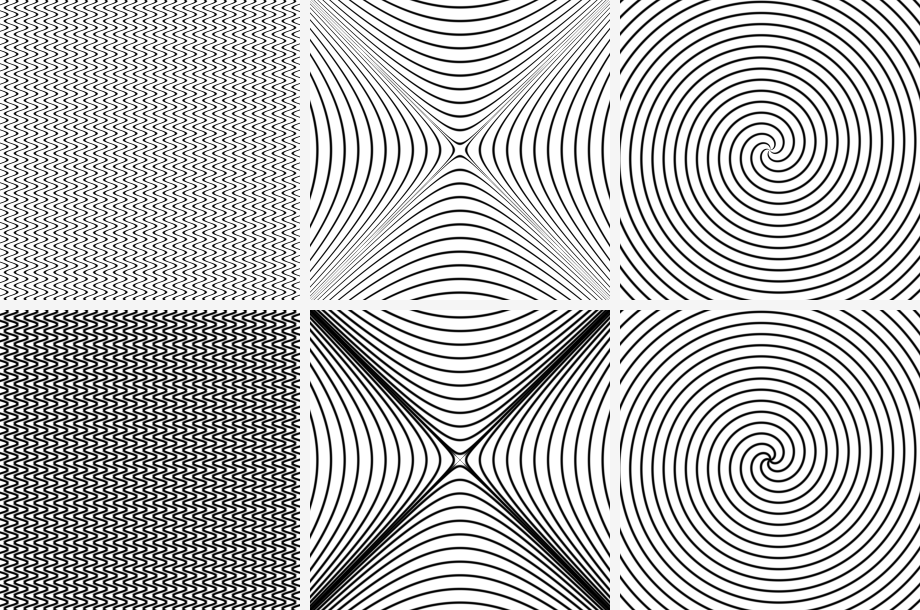
\includegraphics[width=\linewidth]{figures/gradient-compare.png}
  \panelrow{0.32609}{0.01087}{wave, hyperbola, spiral}
  \Description{A two-by-three grid of black-on-white panels: a wave family, a
  hyperbola family and a spiral family, drawn twice. In the top row the strokes fade
  to nothing towards the edges where the curves crowd together; in the bottom row
  those same regions are solid black.}
  \caption{\figlead{A phase residual is not a distance.} Top: for the wave,
  hyperbola and spiral families, what our shader drew was the phase residual,
  undivided.
  Strokes thin by exactly the factor the family is steep by, so the pattern fades
  where it should saturate and the hyperbola's asymptotes disappear. Bottom: the
  same settings with Eq.~\ref{eq:eikonal}. Our shader applied the division for the
  parabola family but not for these three, and the failure is worst where the
  family is densest.}
  \label{fig:gradient}
\end{figure}

The division by $\lVert\nabla\ph\rVert$ in Eq.~\ref{eq:eikonal} converts a phase
residual into a length. It is easy to omit, and we omitted it. Our shader applied
it for the parabola family and not for the wave, hyperbola or spiral, with two
consequences.

The first is cosmetic but severe. Where $\lVert\nabla\ph\rVert>1$, the reported
distance is $\lVert\nabla\ph\rVert$ times too large, so the stroke is thinner by
the same factor. Sweeping each
family over its own slider range on a $1400\times880$ frame
(supplemental material, \S S2) we measure factors up to
$\gradWorstWave$ for the wave and $\gradWorstHyp$ for the hyperbola, with more than
half the frame off by over $10\%$ in both cases. Visually the family pales out
where it steepens and crowds, the opposite of what the geometry does
(Figure~\ref{fig:gradient}).

The second is a correctness bug. Our stroke half-width is
$\mathrm{halfT}=\max(t/2,\,1.15\,\mathrm{px})$, and the floor exists so that a
hairline stays a hairline instead of breaking into speckle when zoomed out
(Section~\ref{sec:zoom}). That floor is a statement about \emph{screen} distance.
Compared against an undivided phase residual it is a statement about phase, and it
guarantees nothing wherever $\lVert\nabla\ph\rVert\neq1$. The steep
families, the ones that most need the floor, are precisely the ones that were
not getting it.

We adopt Eq.~\ref{eq:eikonal} everywhere. One cost: a wave at high amplitude
and frequency now saturates to solid ink, because at those settings its members
genuinely are closer together than a stroke width. That is the correct answer, and
the previous behavior was hiding it.

Eq.~\ref{eq:eikonal} is an eikonal approximation and it is exact only where the
family is locally a foliation with steady gradient. The one family in our
catalog that violates this is the hyperbola, whose gradient blows up on the
asymptote pair (the degenerate $n=0$ level set, where the foliation folds);
the table excludes that member from the family for this reason.

\subsection{Compositing}

Layers composite as ink over paper. With stroke half-width $h_i$ and antialias
band $a$, layer $i$ contributes coverage
\begin{equation}
  \alpha_i(p) = \Big(1-\mathrm{smoothstep}(h_i-a,\;h_i+a,\;d_i(p))\Big)\,o_i,
  \label{eq:alpha}
\end{equation}
and the frame is the running \texttt{mix} of background with each layer's color
at that alpha. For two black layers on white this is the union
$\alpha_1+\alpha_2-\alpha_1\alpha_2$. There is no separate composite pass, no
intermediate texture, and no place in the pipeline where a layer exists as pixels.
$F$ is that union, read on the torus; $\alpha$ is $F\circ\cnt$ after the
stroke profile.

Three properties follow immediately.

\emph{No resolution.} $\cnt$ and $d$ are defined at every real position, so
changing zoom changes only where they are sampled. A moir\'e authored at one scale
is the same moir\'e at another (Section~\ref{sec:zoom}).

\emph{Bounded transitions by construction.} The stroke floor
$h\ge1.15\,\mathrm{px}$ means the ink field's transition band is never narrower
than a pixel, so the energy above the display Nyquist rate is small (not zero:
\S\ref{sec:zoom} measures the residue) without any filtering step. This
approximates what the suppression literature achieves with prefiltering and the
synthesis literature cannot achieve at all: the designed difference component is
kept, and the undesigned beats against a resampling grid are never created
because there is no resampling grid.

\emph{Editability.} Every parameter enters $\cnt$ and $d$ analytically. Moving a
slider does not invalidate a cached raster, because there is none.
